\newpage
\chapter{Interfacing a component model with OASIS3-MCT}
\label{sec_modelinterfacing}

At run-time, the OASIS3-MCT coupling layer supports coupling data
between two components as well as interpolation and transformation
of coupling fields. Different communication techniques have been historically
developed in OASIS. With OASIS3-MCT, communication is performed by MCT based on Message Passing Interface 1 protocol (the keyword \$CHANNEL in the configuration file {\it namcouple} has to be {\tt MPI1}, see chapter \ref{sec_namcouple}). 

For a practical test case using the OASIS3-MCT library, see the sources in
{\tt examples/tutorial} and more details in chapter \ref{sec_compilationrunning}.

To communicate with another component model or to perform I/O actions, a component model needs to be interfaced with the OASIS3-MCT library, which sources can be found in {\tt oasis3-mct/lib/psmile} directory. The OASIS3-MCT library supports:

\begin{itemize}
\item parallel communication between parallel component models,
\item an ability to couple a component on a subset of it's processeses only,
\item automatic sending and receiving actions at appropriate times
 following user's choice indicated in the {\it namcouple},
\item time integration or accumulation of the coupling fields,
\item some transformations such as mapping (interpolation) between grids,
\item I/O actions from/to files.
\end{itemize}

To adapt a component model to OASIS3-MCT, specific calls of
 the following classes have to be implemented in the code:

\begin{enumerate}
\item Initialisation (section \ref{subsubsec_Initialisation})
\item Grid data file definition (section \ref{subsubsec_griddef})
\item Partition definition (section \ref{subsubsec_Partition})
\item coupling-I/O field declaration (section \ref{subsubsec_Declaration})
\item End of definition phase (section \ref{subsubsec_Endofdefinition})
\item coupling-I/O field sending and receiving (section
\ref{subsubsec_sendingreceiving})
\item Termination (section \ref{subsubsec_Termination})
\item Optional auxiliary routines (section \ref{subsubsec_auxroutines})
\end{enumerate}

Finally, in section \ref{subsubsec_Algoritms}, different coupling
algorithms are illustrated and details on how to
reproduce them with OASIS3-MCT are provided. More information on the {\tt LAG} and {\tt SEQ} indices are also given in that section.

\section{Use of OASIS3-MCT library}
\label{subsubsec_Use}
%{Use}

To use OASIS3-MCT library, a user needs to add in his code: 

\begin{itemize}

\item {\tt USE mod\_oasis}

 ** OR **

\item {\tt USE mod\_prism}
 
\end{itemize}

Both use statements are valid and use of just one or the other is recommended in a particular component model. A single use statement now provides all the methods that required multiple use statements in previous OASIS3 versions.  The 
methods, datatypes, and capabilities are identical for both the {\tt mod\_prism} or {\tt mod\_oasis} interfaces.  The only difference is the name of the interface. The interface in module {\tt mod\_prism} is provided for backwards compatability with prior versions of OASIS3. Use of module {\tt mod\_oasis} is now recommended provides access to a set of updated routine names that will continue to evolve in the future, always ensuring backward compatibility.  In the following sections, both the {\tt mod\_prism} and {\tt mod\_oasis} interface names is defined and a single description of the interface arguments is provided. 

\section{Initialisation}
\label{subsubsec_Initialisation}
%{Initialisation}

\subsection{Coupling initialisation}

\begin{itemize}

\item {\tt CALL oasis\_init\_comp        (compid, model\_name, ierror)} 
\item {\tt CALL prism\_init\_comp\_proto (compid, model\_name, ierror)} 

 \begin{itemize}
   \item {\tt compid [INTEGER; OUT]}: component model ID 
   \item {\tt model\_name [CHARACTER*6; IN]}: component model name (as in
  {\em namcouple}) 
   \item {\tt ierror [INTEGER; OUT]}: returned error code.
 \end{itemize}
 
This routine must called by all component processes to initialise the
coupling.\footnote{The model may call MPI\_Init explicitly, but if so, has to
call it before calling {\tt prism\_init\_comp\_proto}; in this case, the
model also has to call MPI\_Finalize explicitly, but only after calling
{\tt prism\_terminate\_proto}.}
\end{itemize}

\subsection{Communicator for internal parallelisation}
\label{subsec_MPI1}

\begin{itemize}
\item {\tt CALL oasis\_get\_localcomm        (local\_comm, ierror )}
\item {\tt CALL prism\_get\_localcomm\_proto (local\_comm, ierror )}

 \begin{itemize}
   \item {\tt local\_comm [INTEGER; OUT]}: value of local communicator
   \item {\tt ierror [INTEGER; OUT]}: returned error code.
 \end{itemize}

  If needed, this routine may be called by the component processes  
  to get the value of a local communicator to be used by the component
  for its internal parallelisation.

  This may be needed as all component models started in a
  pseudo-MPMD mode with MPI1 share automatically the same MPI\_COMM\_WORLD
  communicator.  Another communicator has to be used for the internal
  parallelisation of each component. OASIS3-MCT creates this local
  communicator based on the name given to {\tt oasis\_init\_comp/prism\_init\_comp\_proto} routine; its value is returned
  as the first argument of the routine, {\tt local\_comm}.

%  With CLIM-MPI2, OASIS3 executable spawns the component model executables at the
%  beginning of the run; 
%  the components keep their internal parallelisation context unchanged 
%  with respect to their standalone mode. In this case, calling the 
%  prism\_get\_localcomm\_proto 
%  routine is useless but if called, the communicator MPI\_COMM\_WORLD will be returned as
%  local communicator.
\end{itemize}

\subsection{Coupling through a subset of the component model
  processes}
\label{subsec_subset}

If only a subset of the component processes participate in the coupling (e.g. a component is setup to run on 80 processes but
16 of those processes are associated with a distinct task, like I/O), a communicator gathering only these processes must be defined, with either {\tt oasis/prism\_create\_couplcomm} or \newline {\tt oasis/prism\_set\_couplcomm}.

If such communicator does not exist yet in the code, the component processes should use, to create it: 

\begin{itemize}
\item {\tt CALL oasis\_create\_couplcomm(icpl, local\_comm, coupl\_comm, kinfo)} 
\item {\tt CALL prism\_create\_couplcomm(icpl, local\_comm, coupl\_comm, kinfo)}
\begin{itemize}
\item {\tt icpl [INTEGER; IN]}: coupling process flag
\item {\tt local\_comm [INTEGER; IN]}: MPI communicator with all processes of the component
\item {\tt coupl\_comm [INTEGER; OUT]}: returned MPI communicator gathering only component processes participating in the coupling
\item {\tt kinfo [INTEGER; OUT; OPTIONAL]}: returned error code
\end{itemize}

This routine creates a coupling communicator for a subset of processes. It must be called by all component processes with {\tt icpl=1} for processes participating in the coupling and with {\tt icpl=MPI\_UNDEFINED} for the others. Argument {\tt local\_comm} is the MPI communicator associated with all processes of the component. The new coupling communicator is returned in {\tt coupl\_comm} argument and the internal coupling communicator is also set to that value.  
\end{itemize}

If this communicator already exist in the code, the component should use, to provide it to OASIS3-MCT:  

\begin{itemize} 
\item {\tt CALL oasis\_set\_couplcomm(coupl\_comm, kinfo)}
\item {\tt CALL prism\_set\_couplcomm(coupl\_comm, kinfo)}
\begin{itemize}
\item {\tt coupl\_comm [INTEGER; IN]}: MPI communicator gathering only component processes participating in the coupling
\item {\tt kinfo [INTEGER; OUT; OPTIONAL]}: returned error code
\end{itemize}

This routine allows to provide a local coupling communicator to OASIS3-MCT, given that it already exists in the code. The value of {\tt coupl\_comm} must be the value of this local coupling communicator for the processes participating to the coupling and it must be {\tt MPI\_COMM\_NULL} for processes not involved in the coupling.  
\end{itemize}

These routines should be called after the {\tt oasis\_init\_comp/prism\_init\_comp\_proto}
but before the grid, partition, or coupling field declaration.
All OASIS3-MCT interface routines, besides the grid definition (see
section \ref{subsubsec_griddef}) and the ``puts'' and `` gets'' per se
(see section \ref{subsubsec_sendingreceiving}), are collective and
must be called by all processes.
%\footnote{In fact, the {\tt oasis\_def\_var/prism\_def\_var\_proto} must be %called by at least the root process of the coupler
%communicator but can be called by all processes.}. 
In particular, the
coupling fields sent or received by the component must be declared by
all component processes
with {\tt oasis\_def\_var} / {\tt prism\_def\_var\_proto} (see section \ref{subsubsec_Declaration}), even
if the symbolic names of the variables defined on the processes not involved in the coupling can be
different from the ones defined in the namcouple.
The field partition must also be described across all coupling
processes with {\tt oasis\_def\_partition} / {\tt prism\_def\_partition\_proto} (but with {\tt
  ig\_paral(:)=0} for the processes not involved in the coupling, see
section \ref{subsubsec_Partition}.) 

Here is a coding sample of how to use these routines:
 
\begin{verbatim}
  CALL oasis_init_comp (comp_id, comp_name, ierror )
  CALL oasis_get_localcomm ( localComm, ierror )

  !--- create communicator gathering coupling processes (every other)
  CALL MPI_Comm_Rank ( localComm, mype, ierror )
  couplingpe = .false.
  if (mod(mype,2) == 0) couplingpe = .true. 
  icpl = MPI_UNDEFINED
  if (couplingpe) icpl = 1
  CALL MPI_COMM_Split(localComm,icpl,1,couplComm,ierror)
  !
  !--- provide this communicator to OASIS3-MCT
  CALL oasis_set_couplcomm(couplComm, ierror)
  
  ! The call to MPI_COMM_Split and oasis_set_couplcomm could be replaced by 
  ! CALL oasis_create_couplcomm(icpl,localComm,couplComm,ierror)

  CALL oasis_def_partition ( ... )
  CALL oasis_def_var ( ... )
  CALL oasis_enddef ( ... )

  !--- do loop
     ! ...
     if (couplingpe) CALL oasis_put( ... )
     ! ...
     if (couplingpe) CALL oasis_get( ... )
     ! ...
  !--- enddo

  CALL oasis_terminate ( ... )
\end{verbatim}

\subsection{Separate executable not coupling at all}
\label{subsec_nocpl}

For a model that is launched by oasis as a separate executable but that is NOT coupling at all, 
the only calls that should be made are :

\begin{verbatim}
  CALL oasis_init_comp (comp_id, comp_name, ierror )
  CALL oasis_get_localcomm ( localComm, ierror )   ! optional
  CALL oasis_enddef ( ... )
  CALL oasis_terminate ( ... )
\end{verbatim}

\section{Grid data file definition}
\label{subsubsec_griddef}

With OASIS3-MCT, the grid data files {\em grids.nc, masks.nc} and {\em
  areas.nc} are required only for certain operations (see also
section \ref{subsec_griddata}), i.e.  {\em grids.nc}, and {\em
  masks.nc} for {\tt SCRIPR} (see section
\ref{subsec_interp}) and {\em masks.nc} and {\em areas.nc} 
for {\tt CONSERV} (see section \ref{subsec_cooking}). These grid data files can be
created by the user before the run or can be written directly at run
time by the {\bf master process of each component model} with the following
routines.  These routines can be used by the component models to add
grid fields to the grid files but grid fields
are {\bf never} overwritten in the grid files. These routines have to
be called just after {\tt oasis\_init\_comp}. 

\begin{itemize}

\item {\tt CALL  oasis\_start\_grids\_writing (flag)} or
\item {\tt CALL  prism\_start\_grids\_writing (flag)}
\begin{itemize}
    \item {\tt flag [INTEGER; OUT]}:  not used
  \end{itemize}
  Obsolete in OASIS3-MCT; exists however for upward compatibility.

\vspace{0.2cm}
\item {\tt CALL oasis\_write\_grid (cgrid, nx, ny, lon, lat)} or
\item {\tt CALL prism\_write\_grid (cgrid, nx, ny, lon, lat)}
        
 \begin{itemize}
    \item {\tt cgrid [CHARACTER*4; IN]}: grid name prefix (see
    \ref{subsec_namcouplesecond})
    \item {\tt nx [INTEGER; IN]} : first grid dimension (x)
    \item {\tt ny [INTEGER; IN]} : second grid dimension (y)
    \item {\tt lon [REAL, DIMENSION(nx,ny); IN)} : array of longitudes
      (degrees East) 
    \item {\tt lat [REAL, DIMENSION(nx,ny); IN)} : array of latitudes
    (degrees North)
 \end{itemize}

 Writes the model grid longitudes and latitudes. Longitudes must
 be given in degrees East in the interval -360.0 to 720.0. Latitudes
 must be given in degrees North in the interval -90.0 to 90.0. Note
 that if some grid points overlap, it is recommended to define those
 points with the same number (e.g. 90.0 for both, not 450.0 for one
 and 90.0 for the other) to ensure automatic detection of overlap by OASIS3-MCT
 (which is essential to have a correct conservative remapping
 \texttt{SCRIPR/CONSERV}, see section \ref{subsec_interp}). 

\vspace{0.2cm}
\item {\tt CALL oasis\_write\_corner (cgrid, nx, ny, nc, clon, clat)} or
\item {\tt CALL prism\_write\_corner (cgrid, nx, ny, nc, clon, clat)}

 \begin{itemize}
    \item {\tt cgrid [CHARACTER*4; IN]}: grid name prefix
    \item {\tt nx [INTEGER; IN]} : first grid dimension (x)
    \item {\tt ny [INTEGER; IN]} : second grid dimension (y)
    \item {\tt nc [INTEGER; IN]} : number of corners per grid cell (always 4 in the version)
    \item {\tt lon [REAL, DIMENSION (nx,ny,nc);IN]} : array of corner
    longitudes (in degrees\_East)
    \item {\tt lat [REAL, DIMENSION (nx,ny,nc);IN]} : array of corner
    latitudes (in degrees\_North)
 \end{itemize}

 Writes the grid cell corner longitudes and latitudes
 (counterclockwise sense). Longitudes must be given in degrees East in
 the interval -360.0 to 720.0. Latitudes must be given in degrees
 North in the interval -90.0 to 90.0. Note also that cells larger than
 180.0 degrees in longitude are not supported. Writing of corners is
 optional as corner information is needed only for {\tt
   SCRIPR/CONSERV} (see section \ref{subsec_interp}). If called, needs
 to be called after {\tt oasis/prism\_write\_grid}.

\vspace{0.2cm}
\item {\tt CALL oasis\_write\_mask (cgrid, nx, ny, mask)} or
\item {\tt CALL prism\_write\_mask (cgrid, nx, ny, mask)}

 \begin{itemize}
    \item {\tt cgrid [CHARACTER*4; IN]}: grid name prefix 
    \item {\tt nx [INTEGER; IN]} : first grid dimension (x)
    \item {\tt ny [INTEGER; IN]} : second grid dimension (y)
    \item {\tt mask [INTEGER, DIMENSION(nx,ny) ;IN]} : mask array (be
      careful about the OASIS historical convention (!): 0 = not masked, 1 = masked)
 \end{itemize}
Writes the model grid mask.

\vspace{0.2cm}
\item {\tt CALL oasis\_write\_area (cgrid, nx, ny, area)} or
\item {\tt CALL prism\_write\_area (cgrid, nx, ny, area)}

 \begin{itemize}
    \item {\tt cgrid [CHARACTER*4; IN]}: grid name prefix
    \item {\tt nx [INTEGER; IN]} : first grid dimension (x)
    \item {\tt ny [INTEGER; IN]} : second grid dimension (y)
    \item {\tt area [REAL, DIMENSION(nx,ny); IN]} : array of grid cell areas
 \end{itemize}
Writes of the model grid cell areas. Needed only for {\tt CONSERV}
operation (see section \ref{subsec_cooking}).

\vspace{0.2cm}
\item {\tt CALL prism\_terminate\_grids\_writing()}
\item {\tt CALL oasis\_terminate\_grids\_writing()}

Terminates grids writing (required if some of the above grid writing
routines are called).

\end{itemize}

The creation of the different files is effective in the routine oasis\_enddef.

\section{Partition definition}
\label{subsubsec_Partition}


The coupling fields sent or received by a component model are usually
scattered among the different component processes. With OASIS3-MCT,
all processes exchanging coupling data have to define their local
partition in the global index space. If only a subset of the processes
actually exchange coupling data, the processes not implied in the
coupling have to call this routine to describe a null partition (i.e. with {\tt ig\_paral(:)=0}).

\begin{itemize}

\vspace{0.2cm}
\item {\tt CALL oasis\_def\_partition        (il\_part\_id, ig\_paral, ierror, isize)}
 or 
\item {\tt CALL prism\_def\_partition\_proto (il\_part\_id, ig\_paral, ierror, isize)}

   \begin{itemize}
   \item {\tt il\_part\_id [INTEGER; OUT]}: partition ID 
   \item {\tt ig\_paral [INTEGER, DIMENSION(:), IN]}: vector of
   integers describing the local partition in the global index space; has a different expression depending on the type of the
partition; in OASIS3-MCT, 4 types of partition are supported: Serial (no
partition), Apple, Box, and Orange (see below).
   \item {\tt ierror [INTEGER; OUT]}: returned error code.
   \item {\tt isize [INTEGER, OPTIONAL, IN]}: Optional argument needed if the coupling data us exchanged for only a subdomain of the global grid; in this case, isize must give the total dimension of the grid (total number of points).
   \end{itemize}
\end{itemize} 

\subsection{Serial (no partition)}

This is the choice for a monoprocess model. In this case, we have 
{\tt ig\_paral(1:3)}:
\begin{itemize}
 \item {\tt ig\_paral(1)} = 0 (indicates a Serial ``partition'')
 \item {\tt ig\_paral(2)} = 0
 \item {\tt ig\_paral(3)} = the total grid size.
\end{itemize}

\subsection{Apple partition} 

Each partition is a segment of the global domain, described by its
global offset and its local size. In this case, we have {\tt
ig\_paral(1:3)}:
\begin{itemize}
 \item {\tt ig\_paral(1)} = 1 (indicates an Apple partition)
 \item {\tt ig\_paral(2)} = the segment global offset
 \item {\tt ig\_paral(3)} = the segment local size
\end{itemize}

Figure \ref{apple_partition} illustrates an Apple partition over 3
processes. 
\begin{figure}
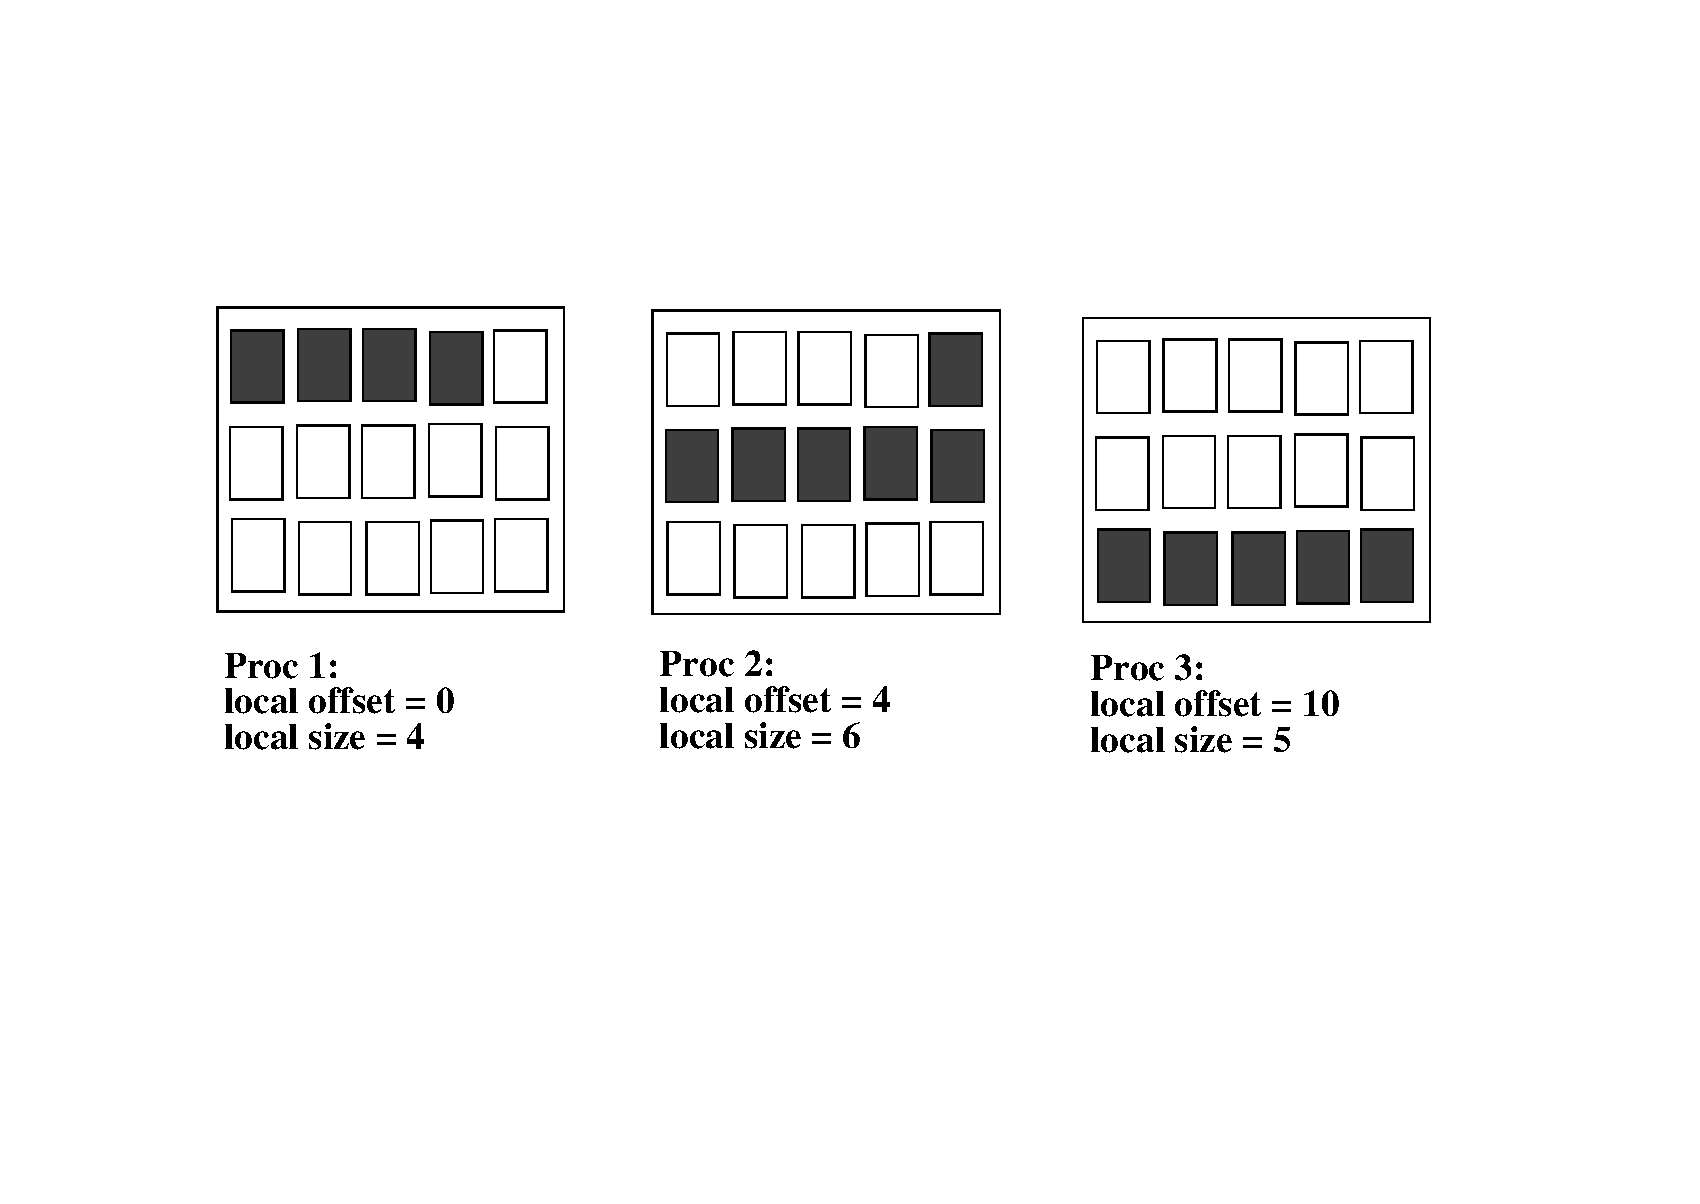
\includegraphics[scale=.6]{figures/apple_new} 
\caption{Apple partition. It is assumed here that the index start at 0 in the upper left corner.}
\label{apple_partition}
\end{figure}


\subsection{Box partition} 

Each partition is a rectangular region of the global domain, described
by the global offset of its upper left corner, and its local extents in the
X and Y dimensions. The global extent in the X dimension must also be
given. In this case, we have {\tt ig\_paral(1:5)}:
\begin{itemize}
 \item {\tt ig\_paral(1)} = 2 (indicates a Box partition)
 \item {\tt ig\_paral(2)} = the upper left corner global offset
 \item {\tt ig\_paral(3)} = the local extent in x
 \item {\tt ig\_paral(4)} = the local extent in y
%\footnote{The maximum
%value of the local extent in y is presently 338; it can be increased
%by modifying the value of {\tt Clim\_MaxSegments} in {\tt
%oasis3/lib/clim/src/mod\_clim.F90} and in {\tt
%oasis3/lib/psmile/src/mod\_prism\_proto.F90} and by recompiling
%OASIS3 and the PSMILe library.}
 \item {\tt ig\_paral(5)} = the global extent in x.
\end{itemize}

Figure \ref{box_partition} illustrates a Box partition over 3
processes.  
 
\begin{figure}
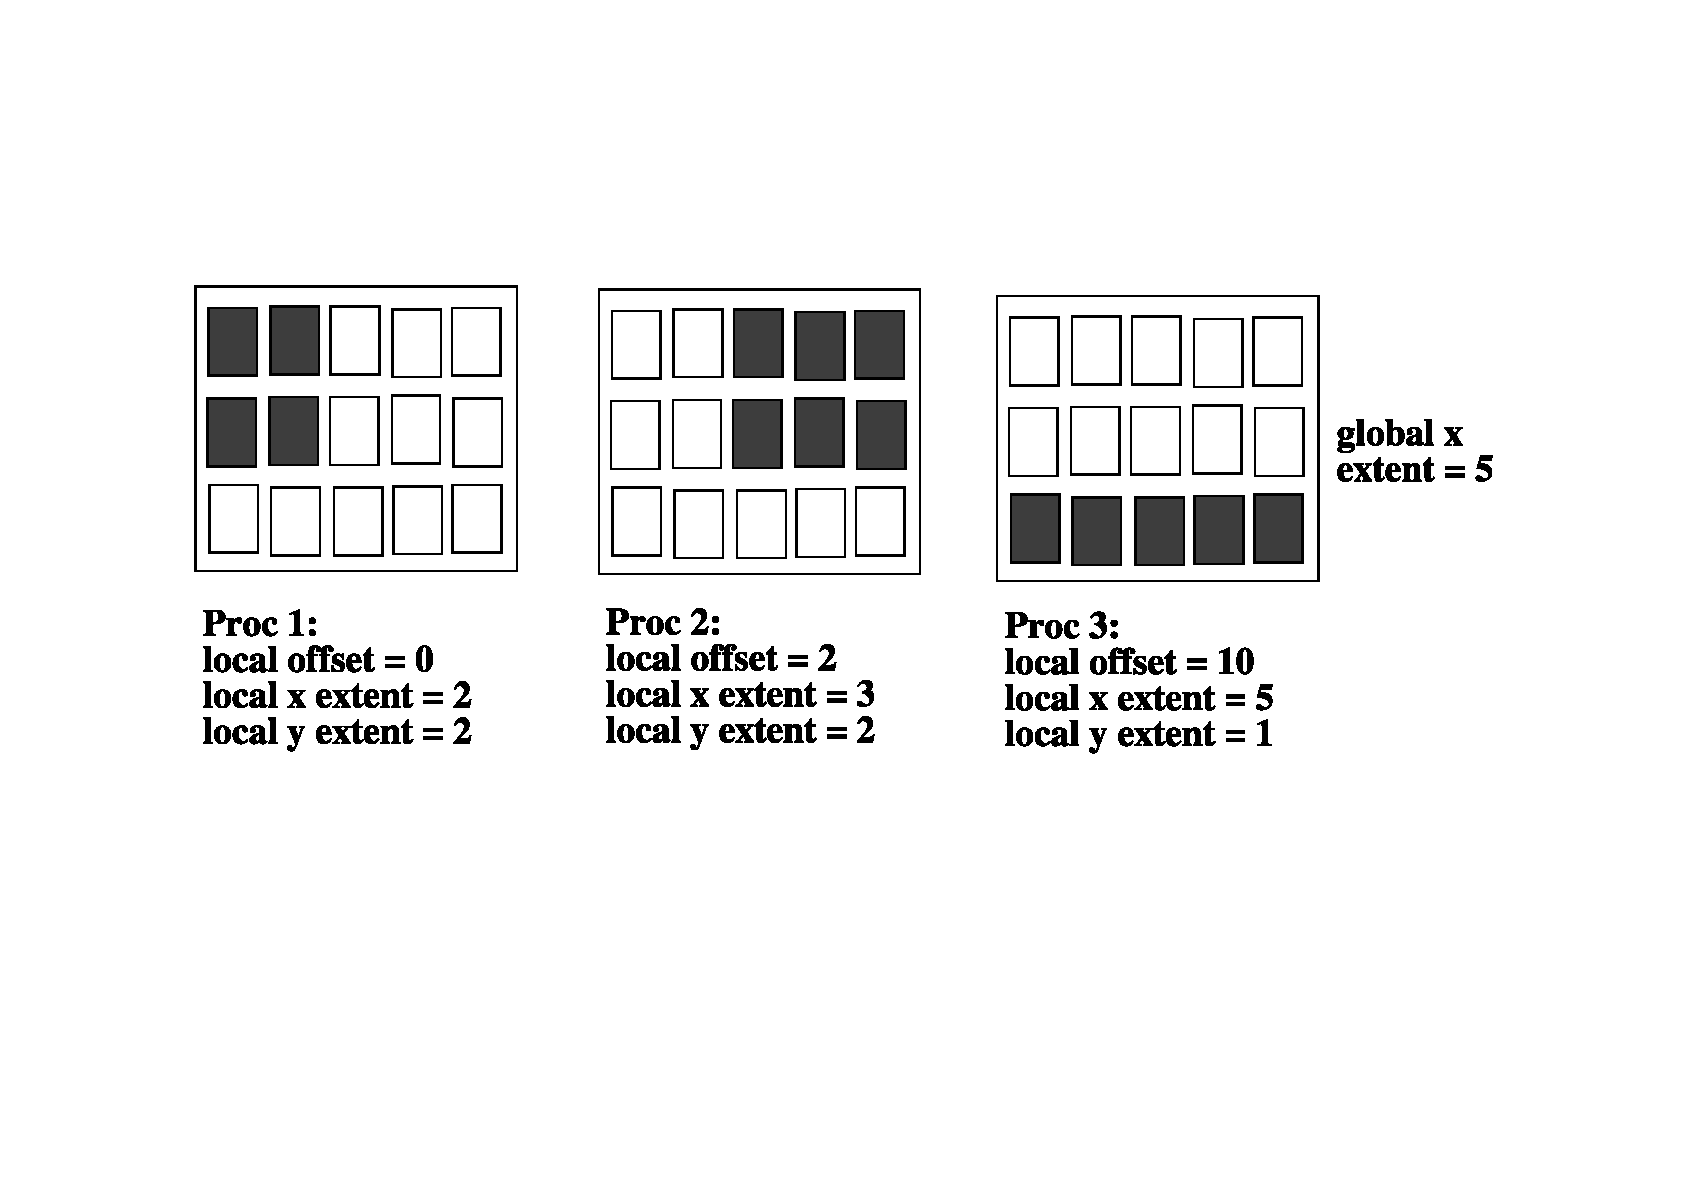
\includegraphics[scale=.6]{figures/box_new} 
\caption{Box partition. It is assumed here that the index start at 0 in the upper left corner.}
\label{box_partition}
\end{figure} 
  
\subsection{Orange partition}

Each partition is an ensemble of segments of the global domain. Each
segment is described by its global offset and its local extent.  In
this case, we have {\tt ig\_paral(1:N)} where {\tt N = 2 + 2*number of
segments}
%\footnote{As for the Box partition, the maximum number of
%segments is presently 338; it can be increased by modifying the value
%of {\tt Clim\_MaxSegments}}.

\begin{itemize}
 \item {\tt ig\_paral(1)} = 3 (indicates a Orange partition)
 \item {\tt ig\_paral(2)} = the total number of segments for the partition (limited to 200 presently, see note for ig\_paral(4) for Box partition above)
 \item {\tt ig\_paral(3)} = the first segment global offset
 \item {\tt ig\_paral(4)} = the first segment local extent
 \item {\tt ig\_paral(5)} = the second segment global offset
 \item {\tt ig\_paral(6)} = the second segment local extent
 \item ...
 \item {\tt ig\_paral(N-1)} = the last segment global offset
 \item {\tt ig\_paral(N)} = the last segment local extent
\end{itemize}

Figure \ref{orange_partition} illustrates an Orange partition with 3 segments
for one process. The other process partitions are not illustrated.

\begin{figure}
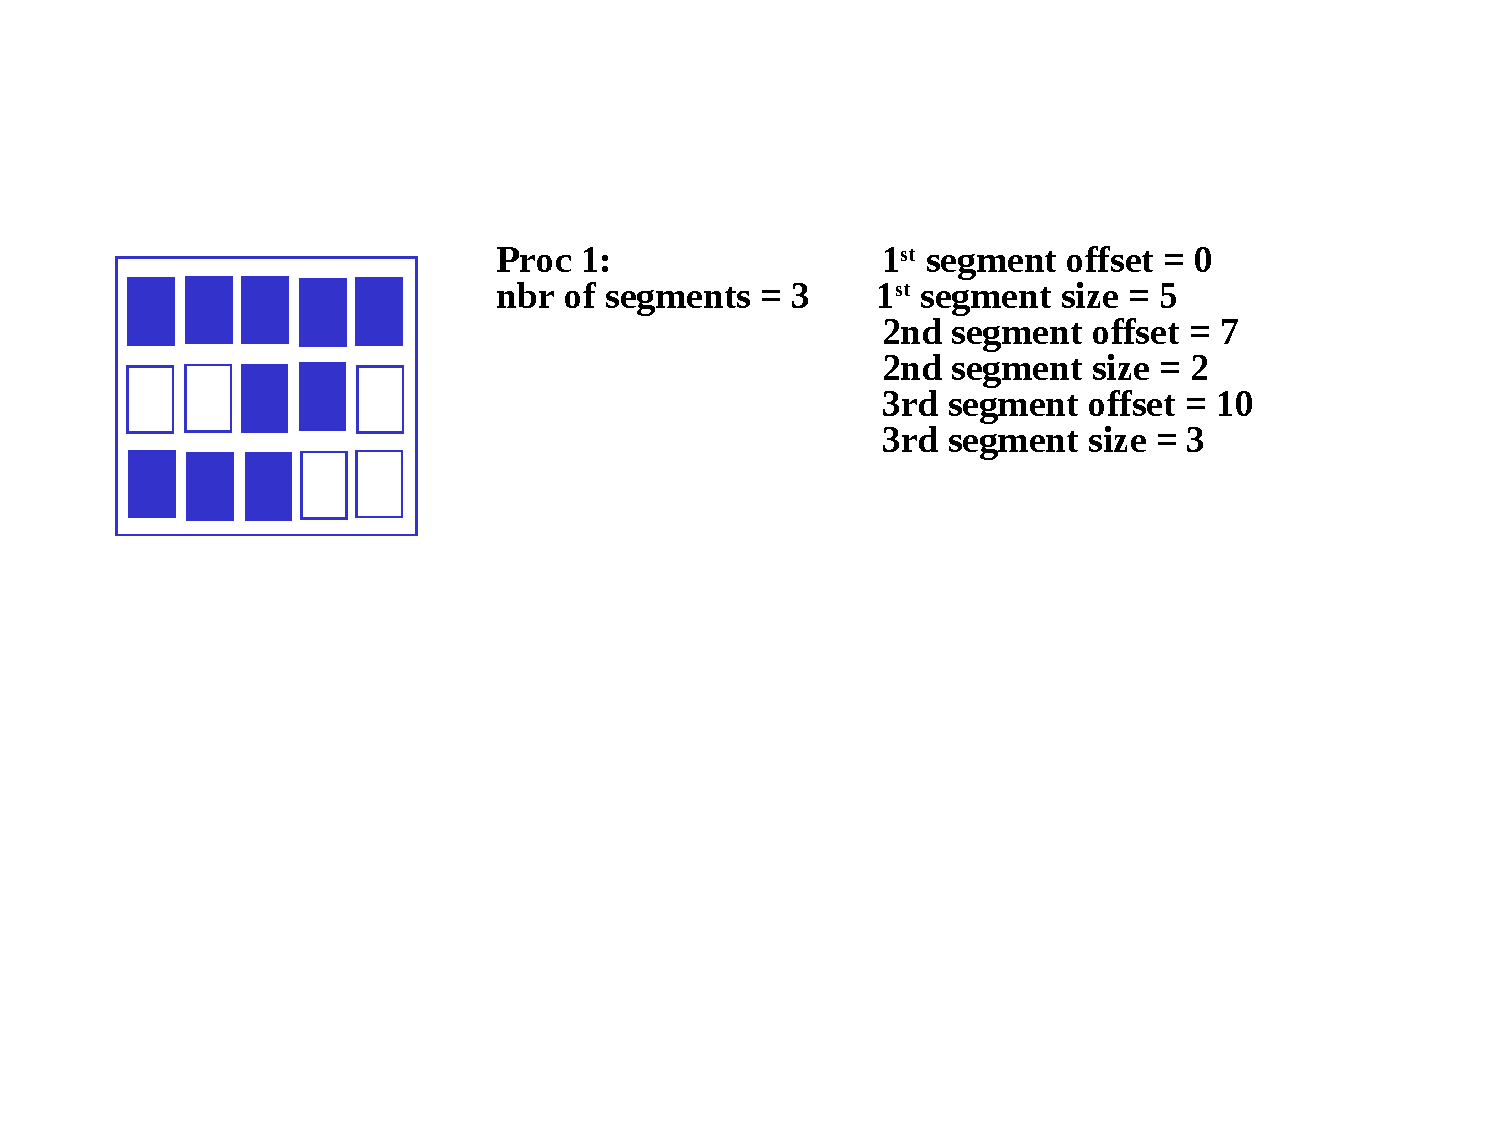
\includegraphics[scale=.6]{figures/orange_new} 
\caption{Orange partition for one process. It is assumed here that the index start at 0 in the upper left corner.}
\label{orange_partition}
\end{figure} 

%{Partition definition}

\section{Coupling field declaration}
 \label{subsubsec_Declaration}

All component processes declares the fields sent
or received by the component during the simulation. This is
  true even for processes not implied in the coupling. 

\begin{itemize}

\item {\tt CALL oasis\_def\_var       (var\_id, name, il\_part\_id,
  var\_nodims, kinout, \newline var\_actual\_shape, var\_type, ierror)} or

\item {\tt CALL prism\_def\_var\_proto(var\_id, name, il\_part\_id,
  var\_nodims, kinout, var\_actual\_shape, var\_type, ierror)}


\begin{itemize}
 \item {\tt var\_id [INTEGER; OUT]}: coupling field ID
 \item {\tt name [CHARACTER*8; IN]}: field symbolic name (as in the
   {\it namcouple})
 \item {\tt il\_part\_id [INTEGER; IN]}: partition ID (see section \ref{subsubsec_Partition})
 \item {\tt var\_nodims [INTEGER, DIMENSION(2); IN]}: var\_nodims(1) is
   the rank of field array (1 or 2); var\_nodims(2) is the number of
   bundles (always 1 for OASIS3-MCT). 
 \item {\tt kinout [INTEGER; IN]}: {\tt OASIS\_In} or {\tt
   PRISM\_In} (i.e. = 15) for fields received by
   the model; {\tt OASIS\_Out}, {\tt PRISM\_Out} (i.e. = 14) for
   fields sent by the model
\footnote{Parameters OASIS\_In,
   PRISM\_In, OASIS\_Out, PRISM\_Out are defined in oasis3-mct/lib/psmile/src/mod\_oasis\_parameters.F90}.
 \item {\tt var\_actual\_shape [INTEGER, DIMENSION(2*var\_nodims(1)); IN]}: 
   vector of integers giving the minimum and maximum index for each
   dimension of the coupling field array; for OASIS3, the minimum
   index has to be 1 and the maximum index has to be the extent of the
   dimension.
 \item {\tt var\_type [INTEGER; IN]}: type of coupling field array;
   put {\tt OASIS\_Real} or {\tt PRISM\_Real} (i.e. = 4) for single or double precision real
   arrays.  All coupling data is treated as double precision in the
   coupling layer, but conversion to or from single precision data
   is supported in the interface.
 \item {\tt ierror [INTEGER; OUT]}: returned error code. 
\end{itemize}
\end{itemize}
%{coupling field declaration}

\section{End of definition phase}
\label{subsubsec_Endofdefinition}
All component processes close the definition phase.
\begin{itemize}
\item {\tt CALL oasis\_enddef       (ierror)}
\item {\tt CALL prism\_enddef\_proto(ierror)}
\begin{itemize}
  \item ierror [INTEGER; OUT]: returned error code.
\end{itemize}
\end{itemize}

%{End of definition phase}

\section{Sending ``put'' and receiving ``get'' actions}
\label{subsubsec_sendingreceiving}

\subsection{Sending a coupling (or I/O) field}
\label{prismput}

In the model time step loop, each process 
sends its part of the coupling (or I/O) field. 

\begin{itemize} 
\item {\tt CALL oasis\_put       (var\_id, date, field\_array, info)}
\item {\tt CALL prism\_put\_proto(var\_id, date, field\_array, info)}
\begin{itemize}
\item {\tt var\_id [INTEGER; IN]}: field ID (from
  corresponding {\tt oasis\_def\_var} / \newline {\tt prism\_def\_var\_proto},
  see section \ref{subsubsec_Declaration})
\item {\tt date [INTEGER; IN]}: number of seconds in the run at the
time of the call (by convention at the beginning of the timestep)
\item {\tt field\_array [REAL, IN]}: coupling (or I/O) field array 
\item {\tt info [INTEGER; OUT]}: returned info code:
   \begin{itemize} 
      \item OASIS\_Sent(=4) if the field was sent to another model 
      \item OASIS\_LocTrans (=5) if the field was only used in a time
       transformation (not sent, not output)
      \item OASIS\_ToRest (=6) if the field was written to a restart file only
      \item OASIS\_Output (=7) if the field was written to an output file only
      \item OASIS\_SentOut (=8) if the field was both written to an output file
       and sent to another model (directly or via OASIS3 main process)
      \item OASIS\_ToRestOut (=9) if the field was written both to a
       restart file and to an output file.
      \item OASIS\_Ok (=0) otherwise and no error occurred.
   \end{itemize}
\end{itemize}
\end{itemize}

To ensure a proper use of the {\tt oasis\_put} / {\tt
  prism\_put\_proto}, one has to take care of the following aspects:

\begin{itemize}

\item This routine may be called by the model at each timestep. The
  convention, for the {\tt date} argument is to indicate the time at
  the beginning of the timestep. The sending is actually performed
  only if the time obtained by adding the field lag ({\tt LAG} in the
  {\em namcouple}) to the {\tt date} corresponds to a time at which it
  should be activated, given the coupling or I/O period indicated by
  the user in the {\it namcouple} (see section \ref{sec_namcouple}). 
\item If the convention for {\tt date} is followed, the first
  coupling of a run should occur at time=0 and the final coupling
  should occur at time = runtime - cpl\_period, where runtime is the
  total time of the run and cpl\_period is the coupling period. 
\item The total run time should match an integer number of coupling
  periods.
\item If a coupling field has a positive lag, the coupling field that
  matches the {\tt oasis\_get} / {\tt prism\_get\_proto} at time=0
  will come from a coupling restart file written by the last active {\tt
  oasis\_put} / {\tt prism\_put\_proto} of the previous run (see
  section \ref{subsubsec_Algoritms}). For a coupling field with a
  positive lag, the coupling restart file (see section
  \ref{subsec_restartdata}) is automatically overwritten by the {\tt
  oasis\_put} / {\tt
    prism\_put\_proto} when the time (i.e. {\tt date+LAG}) equals
  to the total runtime.
%\item A field will not be sent at all if its
%coupling (or I/O) period indicated in the {\it namcouple} is greater
%than the total run time. 
\item If a local time transformation is indicated for the field by the
  user in the {\it namcouple} (INSTANT, AVERAGE, ACCUMUL, T\_MIN or
  T\_MAX, see section \ref{sec_transformations}), it is automatically
  performed and the resulting field is finally sent at the coupling or
  I/O frequency.  For non-instant transformations, partially
  transformed fields will be written to the restart file at the end of
  the run for use on the next model startup; this is a bug fix new in
  OASIS3-MCT.
\end{itemize}

\subsection{Receiving a coupling (or I/O) field}

In the model time stepping loop, each process
receives its part of the coupling field. 

\begin{itemize}
 
\item {\tt CALL oasis\_get       (var\_id, date, field\_array, info)}
\item {\tt CALL prism\_get\_proto(var\_id, date, field\_array, info)}
\begin{itemize}
\item {\tt var\_id [INTEGER; IN]}: field ID (from
  corresponding prism\_def\_var\_proto)
\item {\tt date [INTEGER; IN]}: number of seconds in the run at the
time of the call (by convention at the beginning of the timestep)
\item {\tt field\_array [REAL, OUT]}: I/O or coupling field array 
\item {\tt info [INTEGER; OUT]}: returned info code:
   \begin{itemize} 
      \item OASIS\_Recvd(=3) if the field was received from another model
      \item OASIS\_FromRest (=10) if the field was read from a restart
       file only
      \item OASIS\_Input (=11) if the field was read from an input
       file only
      \item OASIS\_RecvOut (=12) if the field was both received from
       another model and written to an output file
      \item OASIS\_FromRestOut (=13) if the field was both read from a
       restart file and written to an output file
      \item OASIS\_Ok (=0) otherwise and no error occurred.
   \end{itemize}
\end{itemize}
\end{itemize}

This routine may be called by the model at each timestep. The {\tt date}
argument is automatically analysed and the receiving action is actually
performed only if {\tt date} corresponds to a time for which it should
be activated, given the period indicated by the user in the
{\it namcouple}. An exchange at the beginning of the run at time=0 is
expected. 
%A field will not be received at all if its
%coupling or I/O period indicated in the {\it namcouple} is greater
%than the total run time.

\section{Termination}
\label{subsubsec_Termination}

\begin{itemize}

\item {\tt CALL oasis\_terminate       (ierror)}
\item {\tt CALL prism\_terminate\_proto(ierror)}
  \begin{itemize}
  \item {\tt ierror [INTEGER; OUT]}: returned error code.
  \end{itemize}
  All processes of the component model must terminate the coupling by
  calling this routine\footnote{If the process called {\tt
  MPI\_Init} (before calling {\tt oasis\_init\_comp} or {\tt prism\_init\_comp\_proto}), it must
  also call {\tt MPI\_Finalize} explicitly, but only after calling
  {\tt oasis\_terminate\_proto} or {\tt prism\_terminate\_proto}.} (normal termination). 

\end{itemize}

%{Termination}

\section{Auxiliary routines}
\label{subsubsec_auxroutines}

Not all auxiliary routines that were in OASIS3.3 are currently available.

\begin{itemize}
\item {\tt CALL oasis\_abort       (compid, routine\_name, abort\_message)}
\item {\tt CALL prism\_abort\_proto(compid, routine\_name, abort\_message)}
\begin{itemize}
  \item {\tt compid [INTEGER; IN]}: component model ID (from
{\tt oasis\_init\_comp} or \newline {\tt prism\_init\_comp\_proto}) 
  \item {\tt routine\_name[CHARACTER*; IN]}: name of calling routine
  \item {\tt abort\_message[CHARACTER*; IN]}: message to be written out.
\end{itemize}

 If a process needs to abort voluntarily, it should do so by
 calling {\tt oasis\_abort}/{\tt prism\_abort\_proto}. This will ensure a proper
 termination of all processes in the coupled model communicator. This
 routine writes the name of the calling model, the name of the
 calling routine, and the message to the process debug file (see {\tt
   \$NLOGPRT} in section \ref{subsec_namcouplefirst}). 
 This routine cannot be called before {\tt prism\_init\_comp\_proto}.

\vspace{0.2cm} 
\item {\tt CALL oasis\_get\_debug(debug\_value)}
\item {\tt CALL prism\_get\_debug(debug\_value)}
\begin{itemize}
\item {\tt debug\_value [INTEGER; OUT]}: debug value
\end{itemize}

This routine may be called at any time to retrieve the current
OASIS3-MCT internal debug level (see {\tt
\$NLOGPRT} in section \ref{subsec_namcouplefirst}).  This is useful
if the user wants to return the original debug value after changing
it or if a user wants to key off the oasis
debug level for model debug diagnostics.

\vspace{0.2cm} 
\item {\tt CALL oasis\_set\_debug(debug\_value)}
\item {\tt CALL prism\_set\_debug(debug\_value)}
\begin{itemize}
\item {\tt debug\_value [INTEGER; IN]}: debug value
\end{itemize}

This routine may be called at any time to change the debug level in oasis.
This method allows users to vary the debug level at different points
in the model integration.

\vspace{0.2cm} 
\item {\tt CALL oasis\_get\_intercomm(new\_comm, cdnam, kinfo)}
\item {\tt CALL prism\_get\_intercomm(new\_comm, cdnam, kinfo)}
\begin{itemize}
\item {\tt new\_comm [INTEGER; OUT]}: mpi intercomm communicator
\item {\tt cdnam [CHARACTER*; IN]}: other model name 
\item {\tt kinfo [INTEGER; OUT; OPTIONAL]}: returned error code
\end{itemize}

This routine sets up an MPI intercomm communicator between the root
processors of two components, the local component and the component
associated with cdnam.  This must be called by both components at
the same time otherwise a deadlock will occur.  In addition, this call
is collective across the tasks of the two components but other
components are not involved.

\vspace{0.2cm} 
\item {\tt CALL oasis\_get\_intracomm(new\_comm, cdnam, kinfo)}
\item {\tt CALL prism\_get\_intracomm(new\_comm, cdnam, kinfo)}
\begin{itemize}
\item {\tt new\_comm [INTEGER; OUT]}: mpi intracomm communicator
\item {\tt cdnam [CHARACTER*; IN]}: other model name 
\item {\tt kinfo [INTEGER; OUT; OPTIONAL]}: returned error code
\end{itemize}

This routine sets up an MPI intracomm communicator between the root
processors of two components, the local component and the component
associated with cdnam.  This must be called by both components at
the same time otherwise a deadlock will occur.  In addition, this call
is collective across the tasks of the two components but other
components are not involved.
\end{itemize}

\section{Coupling algorithms - SEQ and LAG concepts}
\label{subsubsec_Algoritms}

Using the OASIS3-MCT coupling library, the user has full flexibility to reproduce
different coupling algorithms. In the components, the sending and
receiving routines, respectively {\tt oasis\_put/prism\_put\_proto} and {\tt
   oasis\_get/prism\_get\_proto}, can be called at each model timestep, with the
appropriate {\tt date} argument giving the actual time (at the
beginning of the timestep), expressed in ``number of seconds since the
start of the run'' (see section \ref{prismput}). This {\tt date} argument is automatically analysed
by the coupling library
%\footnote{With the PIPE, SIPC, GMEM and previously with
%the CLIM communication techniques, no such analysis was performed. For
%PIPE, SIPC, and GMEM, the sending actions on the source side would
%automatically match the receiving actions on the target side on a FIFO
%(First In First Out) basis.} 
and depending on the coupling period and the lag (LAG) chosen by the 
user for each coupling field in the configuration file {\it namcouple}, different
coupling algorithms can be reproduced without modifying anything in the
component model codes themselves. 

With OASIS3-MCT, the SEQ index is no longer needed in the {\it namcouple}
input to specify the sequencing order of different coupling fields.
The sequence (SEQ) index in the {\it namcouple} file now provides the coupling 
layer with an ability to detect a deadlock before it happens and exit.

The lag concept and indices are explained in more detail below and some
examples are provided.

\vspace{-0.3cm}
\subsection{The lag concept}
\label{subsub_lag}

The lag (LAG) value tells the coupler to modify the time at which that data
is sent (put) by the amount of the lag.  The lag must be
expressed in ``number of seconds'' and can be positive or
negative but should never be larger (in absolute magnitude) than the
coupling period of any field due to problems with restart-ability and
dead-locking. When a component model calls a {\tt oasis\_put/prism\_put\_proto}, the value of the lag is automatically added to the value of the {\tt date} argument and the ``put'' is actually performed when the sum {\tt date+lag} is a coupling time; in the target component, this ``put'' will match a {\tt oasis\_get/prism\_get\_proto} for which the {\tt date} argument is the same coupling time.
%A positive lag indicates the
%put will occur sooner than zero lag and a negative lag tells the coupler
%to send the data later than zero lag.
The lag only shifts the time data is sent.  It cannot be used to shift the time data is received yet.
 
When the lag is positive, a restart file must be available to initiate the coupling and in those cases, the restart file is then updated at the end of the run.  A positive lag acts like a send occurred before the model started. In fact, for a field with positive lag, the source component model automatically reads the field in the restart file during the coupling initialization phase (below the {\tt oasis\_enddef/prism\_enddef\_proto}) and send the data to match the {\tt oasis\_get/prism\_get\_proto} performed at time=0 in the target component model. The final coupling
data on the source side will then be automatically written to the restart file for use in the next run.  

When there is a lag, the first and last instance of the source field
in the debug netCDF file (EXPOUT fields, see section
\ref{subsec_namcouplesecond}) always correspond respectively to the field read from and written to the restart file.
 
  \begin{enumerate}

  \item LAG concept first example
 
  A first coupling algorithm, exploiting the LAG concept, is
  illustrated on figure \ref{fig:lag_concept_1}. 

  On the 4 figures in this section, short black arrows correspond to {\tt
  oasis\_put/prism\_put\_proto} or {\tt oasis\_get/prism\_get\_proto} called in the component model
  that do not lead to any ``put" or receiving action;
  long black arrows correspond to {\tt oasis\_put/prism\_put\_proto} or \break {\tt
  oasis\_get/prism\_get\_proto} called in the component models that do
  actually lead to a ``put" or ``get'' action;
  long red arrows correspond to {\tt oasis\_put/prism\_put\_proto} or \break {\tt
  oasis\_get/prism\_get\_proto} called in the component models that lead to a
  reading or writing of the coupling field from or to a coupling
  restart file.

\begin{figure}
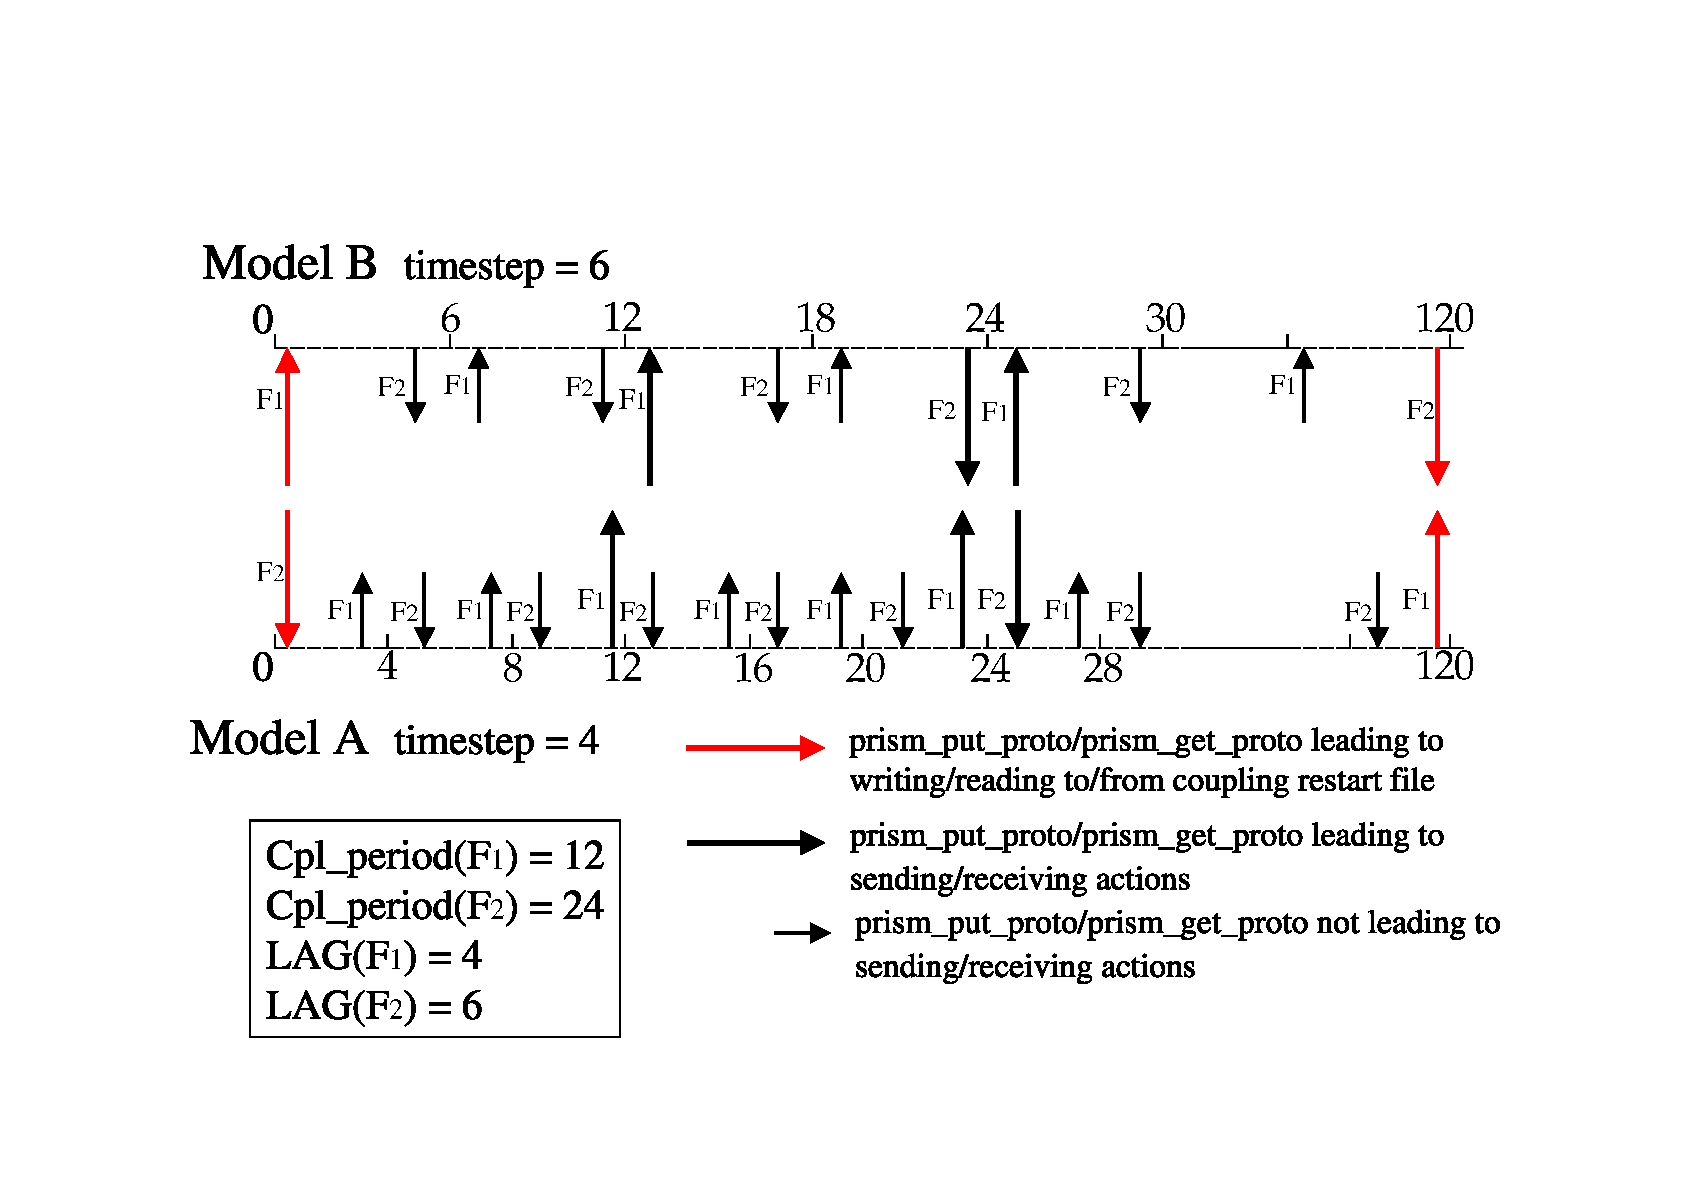
\includegraphics[scale=.6]{figures/fig_lag_concept_1}
\caption{LAG concept first example} 
\label{fig:lag_concept_1}
\end{figure}

  During a coupling timestep, model A receives $F_2$ and then sends $F_1$; its
  timestep length is 4. During a coupling timestep, model B receives $F_1$
  and then sends $F_2$; its timestep length is 6.  $F_1$ and $F_2$
  coupling periods are respectively 12 and 24. If $F_1$/$F_2$ ``put"
  action by model A/B was used at a coupling timestep to match the
  model B/A ``get" action, a deadlock would occur as both models
  would be initially waiting on a ``get" action. To prevent this,
  $F_1$ and $F_2$ produced at the timestep before have to be used to
  match respectively the model B and model A ``get" actions.

  This implies that a lag of respectively 4 and 6 seconds must be
  defined for $F_1$ and $F_2$. For $F_1$, the {\tt oasis\_put/prism\_put\_proto}
  performed at time 8 and 20 by model A will then lead to ``put" actions
  (as 8 + 4 = 12 and 20 + 4 = 24 which are coupling periods) that
  match the ``get" actions performed at times 12 and 24 below the {\tt
  oasis\_get/prism\_get\_proto} called by model B.  For $F_2$, the {\tt
  oasis\_put/prism\_put\_proto} performed at time 18 by model B then leads to
  a ``put" action (as 18 + 6 = 24 which is a coupling
  period) that matches the ``get" action performed at time 24
  below the {\tt oasis\_get/prism\_get\_proto} called by model A.

  At the beginning of the run, as their LAG index is greater than 0,
  the first {\tt oasis\_get/prism\_get\_proto} of $F_1$ and $F_2$ will automatically 
  be fulfilled with fields read from their respective coupling restart files. The user
  therefore has to create those coupling restart files before the first
  run in the experiment. At the end of the run, $F_1$
  having a lag greater than 0, is automatically written to its
  coupling restart file below the last $F_1$ {\tt oasis\_put/prism\_put\_proto} as the
  {\tt date+lag} equals the total run time. The analogue is true
  for $F_2$. These
  values will automatically be read in at the beginning of the next
  run below the respective {\tt oasis\_get/prism\_get\_proto}.

  \item LAG concept second example

  A second coupling algorithm exploiting the LAG concept is
  illustrated on figure \ref{fig:lag_concept_2}. During its timestep,
  model A receives $F_2$, sends $F_3$ and then $F_1$; its timestep
  length is 6. During its timestep, model B receives $F_1$, receives
  $F_3$ and then sends $F_2$; its timestep length is also 6.  $F_1$,
  $F_2$ and $F_3$ coupling periods are both supposed to be equal to
  12.
 
\begin{figure}
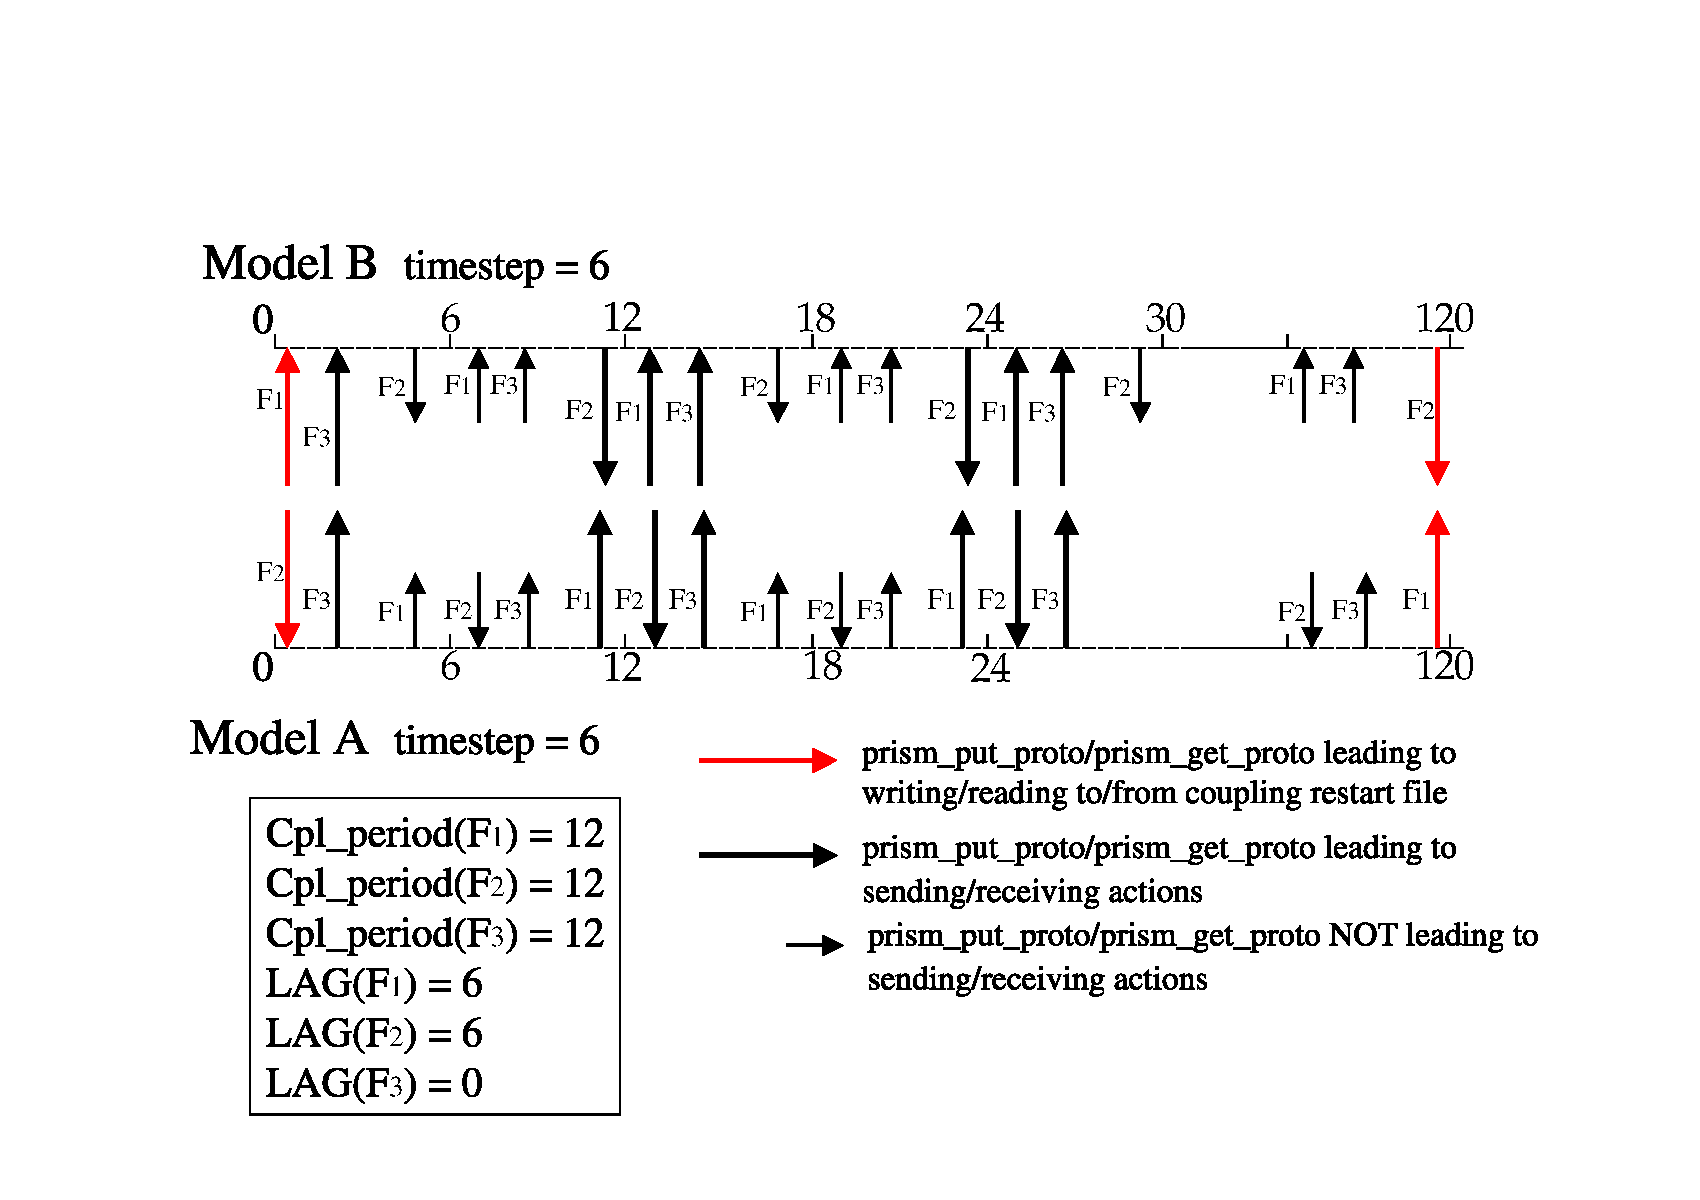
\includegraphics[scale=.6]{figures/fig_lag_concept_2} 
\caption{LAG concept second example} 
\label{fig:lag_concept_2}
\end{figure}

  For $F_1$ and $F_2$ the situation is similar to the first
  example. If $F_1$/$F_2$ ``put" action by model A/B was used at a
  coupling timestep to match the model B/A ``get" action, a
  deadlock would occur as both models would be waiting on a ``get"
  action. To prevent this, $F_1$ and $F_2$ produced at the timestep
  before have to be used to match the model A and model B ``get"
  actions, which means that a lag of 6 must be defined for both $F_1$
  and $F_2$. For both coupling fields, the {\tt oasis\_put/prism\_put\_proto}
  performed at times 6 and 18 by the source model then lead to ``put"
  actions (as 6 + 6 = 12 and 18 + 6 = 24 which are coupling periods)
  that match the ``get" action performed at time 12 and 24 below
  the {\tt oasis\_get/prism\_get\_proto} called by the target model.

  For $F_3$, sent by model A and received by model B, no lag
  needs to be defined: the coupling field produced by model A at the
  coupling timestep can be ``consumed'' by model B without causing a
  deadlock situation.

  As in the first example, the {\tt oasis\_get/prism\_get\_proto} performed at
  the beginning of the run for $F_1$ and $F_2$, will automatically receive data read from their coupling restart files, and the last {\tt
  oasis\_put/prism\_put\_proto} performed at the end of the run automatically
  write them to their coupling restart file. For $F_3$, no coupling
  restart file is needed nor used as at each coupling period the
  coupling field produced by model A can be directly ``consumed'' by
  model B.

  We see here how the introduction of appropriate LAG indices results in
  ``get" in the target model,
  coupling fields produced by the
  source model the timestep before; this is, in some coupling
  configurations, essential to avoid deadlock situations.

  \end{enumerate}

\vspace{-0.3cm}
\subsection{The sequence concept}
\label{subsec_sec}

The order of coupling operations in the system is determined solely
by the order of calls to send (put) and receive (get) data in the models
in conjunction with the setting of the lag in the {\it namcouple}.  Data that is
received (get) is always blocking while data that is sent (put) is non-blocking
with respect to the model making that call.  It is possible
to deadlock the system if the relative orders of puts and gets in different
models are not compatible. 

With OASIS3-MCT, the sequence (SEQ) index in the {\it namcouple} file now provides the coupling 
layer with an ability to detect a deadlock before it happens and exit. 
It does this by tracking the order of get and put calls in
models compared to the SEQ specified in the {\it namcouple}.  If there are any
inconsistencies, the model will abort gracefully with a useable error
message before the system deadlocks.  If there are any coupling dependencies
in the system, use of the SEQ index is recommended for diagnosis but
has no impact on the ultimate solution and is NOT required.

Take the following two examples.  In both examples, there are two
models, each ``put" a field to the other at every coupling period
without any lags.  In the first case, there is no dependency and 
each model sends (puts) the data first and then receives the data
second at each timestep.

\begin{verbatim}
     model1        model2
     ------        ------
    put(fld1)     put(fld2)
    get(fld2)     get(fld1)
\end{verbatim}

The put from model1 for fld1 is received by the get in model2 and the
put from model2 for fld2 is received by the get in model1.  In this case,
there is no sequencing dependency and the value of SEQ must be
identical (or unset) in the {\it namcouple} description of the fld1
and fld2 coupling.  If SEQ is set to 1 for fld1 and 2 for fld2 in this case, then
the model will abort because at runtime, the coupling will detect, in model 2, that 
fld2 was sent before fld1 was received which is out of sequence
as defined by the SEQ settings.

In the next example, there is a dependency in the sequencing.

\begin{verbatim}
     model1        model2
     ------        ------
    put(fld1)     get(fld1)
                  fld2=g(fld1)
    get(fld2)     put(fld2)
\end{verbatim}

In model2, fld2 depends on fld1.  If this dependency is known, then
there is a benefit in using SEQ=1 for fld1 and SEQ=2 for fld2.  At
runtime, if the sequencing of both model1 and model2 do not match
the above diagram, the model will abort gracefully.  For instance,
if model2 has the dependency shown above but model1 does not have
consistent ordering of the put and get as required by model2,
then if SEQ is unused, the model will deadlock and hang.  If SEQ
is set properly, the coupling layer will detect that the required
sequence has not been followed and will exit gracefully with an
error message.  

Again, the SEQ namecouple setting is only diagnostic and is
not required.



